%%%%%%%%%%%%%%%%%%%%%%%%%%%%%%%%%%%%%%%%%%%%%%%%%%%%%%%%%%%%%%%%%%%%%%%%%%%%%%%%
%2345678901234567890123456789012345678901234567890123456789012345678901234567890
%        1         2         3         4         5         6         7         8

%\documentclass[journal,transmag]{IEEEtran}% Comment this line out if you need a4paper

\documentclass[10pt, conference]{ieeeconf}      % Use this line for a4 paper

\IEEEoverridecommandlockouts                              % This command is only needed if 
                                                          % you want to use the \thanks command

%\overrideIEEEmargins                                      % Needed to meet printer requirements.

% See the \addtolength command later in the file to balance the column lengths
% on the last page of the document

% The following packages can be found on http:\\www.ctan.org
%\usepackage{graphics} % for pdf, bitmapped graphics files
%\usepackage{epsfig} % for postscript graphics files
%\usepackage{mathptmx} % assumes new font selection scheme installed
%\usepackage{times} % assumes new font selection scheme installed
%\usepackage{amsmath} % assumes amsmath package installed
%\usepackage{amssymb}  % assumes amsmath package installed



\usepackage{amsmath,amssymb}

\usepackage{tabularx}
\usepackage{tikz,hyperref,graphicx,units,subfig}
\usepackage{subfig}
\usepackage{benktools}
\usepackage{caption}
\usepackage{epstopdf}
\renewcommand{\captionfont}{\footnotesize}
\usepackage{sidecap,wrapfig}
\usepackage[ruled,vlined]{algorithm2e}
\DeclareMathOperator*{\argmin}{arg\,min}
\DeclareMathOperator*{\argmax}{arg\,max}
\newcommand{\abs}[1]{\lvert#1\rvert} 
\newcommand{\norm}[1]{\lVert#1\rVert}
%\newcommand{\suchthat}{\mid}
\newcommand{\suchthat}{\ \big|\ }
\newcommand{\ba}{\mathbf{a}}
\newcommand{\bb}{\mathbf{b}}
\newcommand{\bc}{\mathbf{c}}
\newcommand{\bd}{\mathbf{d}}
\newcommand{\bg}{\mathbf{g}}
\newcommand{\bj}{\mathbf{j}}
\newcommand{\bn}{\mathbf{n}}
\newcommand{\bp}{\mathbf{p}}
\newcommand{\bw}{\mathbf{w}}
\newcommand{\bt}{\mathbf{t}}
\newcommand{\by}{\mathbf{y}}
\newcommand{\bx}{\mathbf{x}}
\newcommand{\bz}{\mathbf{z}}
\newcommand{\bbf}{\mathbf{f}}
\newcommand{\bzero}{\mathbf{0}}
\newcommand{\bG}{\mathbf{G}}
\newcommand{\bA}{\mathbf{A}}
\newcommand{\bW}{\mathbf{W}}
\newcommand{\bX}{\mathbf{X}}
\newcommand{\mX}{\mathcal{X}}
\newcommand{\mD}{\mathcal{D}}
\newcommand{\mG}{\mathcal{G}}
\newcommand{\mN}{\mathcal{N}}
\newcommand{\mW}{\mathcal{W}}
\newcommand{\mF}{\mathcal{F}}
\newcommand{\bZ}{\mathbf{Z}}

\newcommand{\bfc}{W}
\newcommand{\Qinf}{Q_{\infty}}
\newcommand{\st}[1]{_\text{#1}}
\newcommand{\rres}{r\st{res}}
\newcommand{\pos}[1]{(#1)^+}
\newcommand{\depth}{\operatorname{depth}}
\newcommand{\dist}{\operatorname{dist}}
\newcommand{\convhull}{\operatorname{ConvexHull}}
\newcommand{\minksum}{\operatorname{MinkowskiSum}}

\newcommand{\specialcell}[2][c]{ \begin{tabular}[#1]{@{}c@{}}#2\end{tabular}}

\newcommand\independent{\protect\mathpalette{\protect\independenT}{\perp}}
\def\independenT#1#2{\mathrel{\rlap{$#1#2$}\mkern2mu{#1#2}}}

\newcolumntype{L}[1]{>{\RaggedRight\hspace{0pt}}p{#1}}
\newcolumntype{R}[1]{>{\RaggedLeft\hspace{0pt}}p{#1}}

\title{\LARGE \bf
Multi-Armed Bandit Models for 2D Grasp Planning with Uncertainty}
%Multi-Arm Bandit Models for 2D Sample-Based Grasp Planning with Uncertainty}


\author{Michael Laskey$^1$, Jeff Mahler$^1$, Zoe McCarthy$^1$,  Florian T. Pokorny$^1$, Sachin Patil$^1$,\\ Jur van den Berg$^4$,  Danica Kragic$^3$, Pieter Abbeel$^1$, Ken Goldberg$^2$% <-this % stops a space
\thanks{$^1$Department of Electrical Engineering and Computer Sciences; {\small \{mdlaskey, jmahler, zmccarthy,
ftpokorny, sachinpatil, pabbeel\}@berkeley.edu}}%
\thanks{$^2$Department of Industrial Engineering and Operations Research and Department of Electrical Engineering and Computer Sciences; {\small goldberg@berkeley.edu}}%
\thanks{$^{1-2}$ University of California, Berkeley;  Berkeley, CA 94720, USA}%
\thanks{$^3$Computer Vision and Active Perception Lab, Centre for Autonomous Systems, School of Computer Science and
Communication, KTH Royal Institute of Technology, Stockholm, Sweden; {\small dani@kth.se}}%
\thanks{$^4$Google; Amphitheatre Parkway, Mountain View, CA 94043, USA; {\small jurvandenberg@gmail.com}}%
} 

\newtheorem{theorem}{Theorem}

\begin{document}



\maketitle
\thispagestyle{empty}
\pagestyle{empty}


%%%%%%%%%%%%%%%%%%%%%%%%%%%%%%%%%%%%%%%%%%%%%%%%%%%%%%%%%%%%%%%%%%%%%%%%%%%%%%%%

\begin{abstract}
For applications such as warehouse order fulfillment, robot grasps must be robust to uncertainty arising from sensing,
mechanics, and control.  One way to achieve robustness is to evaluate the performance of candidate grasps by sampling
perturbations in shape, pose, and gripper approach and to compute the probability of force closure for each candidate to
identify a grasp with the highest expected quality. Since evaluating the
quality of each grasp is computationally demanding, prior work has turned to cloud computing. To improve computational efficiency and to extend this work, we consider how
Multi-Armed Bandit (MAB) models for optimizing decisions can be applied in this context. We formulate robust grasp
planning as a MAB problem and evaluate convergence times towards an optimal grasp candidate using 100 object shapes from
the Brown Vision 2D Lab Dataset with 1000 grasp candidates per object. We consider the case where shape uncertainty is represented as a Gaussian process implicit surface (GPIS) with Gaussian uncertainty in pose, gripper approach angle, and coefficient of friction. 
We find that Thompson Sampling and the Gittins index MAB methods converged to within 3\% of the optimal grasp up to 10x faster than uniform allocation and 5x faster than iterative pruning. 
\end{abstract}


%%%%%%%%%%%%%%%%%%%%%%%%%%%%%%%%%%%%%%%%%%%%%%%%%%%%%%%%%%%%%%%%%%%%%%%%%%%%%%%%

\section{Introduction}


%\vspace{10pt}
%\todo{Get High res GPIS visualizations, Incorporate next round of feedback}

Consider a robot fulfilling orders in a warehouse, where it encounters new consumer products and must handle them quickly.
While planning grasps using analytic methods requires knowledge of contact locations and surface normals,
a robot may not be able to measure these quantities exactly due to sensor imprecision and missing data, which could result from occlusions, transparency, or highly reflective surfaces. 

% \begin{figure}%
%     \centering
% %     \subfloat{{\includegraphics[width=8cm]{figures/cup.jpg} }}%
% %       \qquad
  
%      \subfloat{{\includegraphics[width=8.5cm]{matlab_figures/pfc.eps} }}%
   
%     \caption{ Comparison of the current average probability of force closure vs. the stopping time $T_s$. The plots are averaged over 100 shapes randomly drawn from the Brown Vision 2D Lab Dataset \cite{brown} with $|G|=1000$ for each shape.  We demonstrate this for Thompson, Gittins, Monte-Carlo and the approach of Kehoe et al \cite{kehoe2012toward}. We also plot the average probability of force closure for the estimated optimal grasp evaluated using Monte-Carlo sampling. Empirically, it appears that Thompson and Gittins converge to the optimal solution at a faster rate, which is desired for an anytime algorithm.   }%
%     \label{fig:rot_shapes}%
% \end{figure}

\begin{figure}%
    \centering
     \subfloat{{\includegraphics[scale=1]{matlab_figures/pfc-01.jpg} }}%

     \caption{Number of samples (i.e. iterations of arm pulls) versus the normalized probability of force closure $P_F$ for the best estimated grasp 
        after $t$ samples, $P_F(\Gamma_{\bar{k}, t})$, out of 1000 candidate grasps using uniform allocation, iterative pruning (eliminating candidates that perform poorly on initial samples), and our proposed Multi-Armed Bandit (MAB) algorithms (Gittins indices and Thompson Sampling).
    %We evaluated performance on 100 objects randomly selected from from the Brown Vision 2D Lab Dataset \cite{brown} with 1000 uniformly distributed candidate grasp plans.
    The normalized $P_F$ is given by the ratio of $P_F(\Gamma_{\bar{k}, t})$ to the highest $P_F$ value in the candidate
    grasp set $P_F(\Gamma^*)$ averaged over 100 independent runs on randomly selected objects from the Brown Vision 2D Dataset \cite{brown}.
    The highest quality grasp was determined by brute force search over all candidate grasps (which requires 10x more
    iterations than all methods shown)~\cite{kehoe2012toward}.
    Uniform allocation and iterative pruning converge to within 3$\%$ of the highest quality grasp (the dashed grey line) in approximately 40,000 and 20,000 iterations, respectively. In comparison, the MAB methods both converge in approximately 4,000 iterations. 
%    $P_F(\Gamma_{\bar{k}})$ (ratio of $P_F(\Gamma_{\bar{k}})$ to $P_F(\Gamma^*)$)
%    
%    Normalized grasp quality over time of the returned grasp for 4 sample-based planning methods.  Normalization divides the current quality of grasp, $P_F(\Gamma_{\bar{k}})$ returned by the highest probability of force closure in the candidate grasp set $P_F(\Gamma^*)$. The highest quality grasp was determined by brute force search over all candidate grasps (which required 10x  more time than any of these methods \cite{kehoe2012toward}).  Data is based on 100 objects randomly selected from from the Brown Vision 2D Lab Dataset \cite{brown} with 1000 uniformly distributed candidate grasp plans. Monte Carlo methods such as Uniform sampling and iterative pruning (eliminating candidates that perform poorly on initial samples) eventually converge to within 3$\%$ of the optimal (the dashed grey line), requiring approximately 40,000 and 20,000 iterations.  Two Multi-Arm Bandit methods perform significantly better, converging after only 4000 iterations..
	}
    \label{fig:grasp_quality}
\end{figure}

A common measure of grasp quality is force closure, the ability to resist external forces and torques in arbitrary directions~\cite{li1988task}. To cope with uncertainty, recent work has explored computing the probability of force closure given uncertainty in pose~\cite{christopoulos2007handling, kim2012physically, weisz2012pose} and object shape~\cite{kehoe2012estimating, mahler2015gp}.
To compute the probability of force closure, Monte-Carlo integration over sampled perturbations in the uncertain
quantities can be applied~\cite{christopoulos2007handling,kehoe2012toward, kim2012physically, weisz2012pose}. However,
performing Monte-Carlo integration for each candidate grasp hypothesis is computationally expensive.  Past work has
looked at leveraging cloud computing to parallelize this computation in order to overcome this problem and proposed a heuristic for adaptive sampling known as iterative pruning~\cite{kehoe2012estimating,kehoe2012toward,kehoe2015survey}.
In this work, we aim to extend these methods by reducing the number of samples needed to converge to a high-quality grasp.  

Our main contribution is formulating the grasp selection problem as a Multi-Armed Bandit (MAB) and showing that it is possible to
allocate sampling effort to grasps with an estimated higher probability of force closure~\cite{barto1998reinforcement,
lai1985asymptotically, robbins1985some}. A standard MAB has a set of possible options, or
`arms'~\cite{barto1998reinforcement} that each return a numeric reward from a stationary distribution. The goal in a
MAB problem is to  select a sequence of arm pulls to maximize the expected reward. We formulate the problem of ranking a
set of candidate grasps according to a quality metric in the presence of uncertainty as a MAB problem and consider the
MAB algorithm as an anytime algorithm that terminates either once a user-defined confidence level is met or at a given stopping time. 

We study this formulation using probability of force closure~\cite{christopoulos2007handling,  kehoe2012toward,weisz2012pose} as a quality metric under uncertainty in pose, shape, gripper approach, and friction coefficient. 
We model shape uncertainty using Gaussian process implicit surfaces (GPISs), a Bayesian representation of shape uncertainty that has been used in various robotic applications~\cite{dragiev2011, hollinger2013}. 
Uncertainty in pose is modeled as a normal distribution around the orientation and 2D position of the object while
uncertainty in grasp approach is modeled as a normal distribution around the center and angle of the grasp axis for a
parallel jaw gripper. We furthermore model uncertainty in friction coefficient as a normal distribution around an expected friction coefficient.

We compare Thompson sampling and Gittins indices, two popular algorithms for solving the MAB problem,
against uniform allocation and an adaptive sampling method known as iterative pruning, which iteratively reduces the set
of candidate grasps based on the sample mean~\cite{kehoe2012toward},
in terms of the number of samples needed to find a grasp with highest estimated probability of force closure on objects in the Brown Vision 2D Dataset, a dataset of 2D planar objects~\cite{brown, christopoulos2007handling}. Our simulation results show that Thompson Sampling, a MAB algorithm, required $5$x fewer samples than iterative
pruning and $10$x fewer samples than uniform allocation to determine a grasp within $3\%$ of the estimated highest probability of force closure
grasp among a set of 1000 grasp candidates per object and averaged over 100 objects.

%\todo{Should we say 10x over uniform, or up to 10x improvment, or 5x over iterative pruning? 
%Florian: be consistent with claim in abstract}

%in the set of 1000 randomly selected grasps averaged over 100 objects. 

%by dividing the arms into $M$ subset,where $M$ is the number of available cores, and solving each MAB problem separately\cite{glazebrook2000index}. 


\section{Related Work}

Many works on grasp planning focus on finding grasps by maximizing a grasp quality metric. Grasp quality is often measured by the ability to resist external perturbations to the object in wrench space~\cite{ferrari1992, miller2004graspit}. For example, Liu et al. used gradients on grasp metrics to guide a mutli-fingered hand towards a grasp \cite{liu2004quality}. Analytical quality metrics typically assume precisely known object shape, object pose, and locations of contact~\cite{cheong2011output, ciocarlie2009}. Work on grasping under uncertainty has considered uncertainty in the state of a robotic gripper~\cite{goldberg1990bayesian, stulp2011learning} and uncertainty in contact locations with an object~\cite{zheng2005}. Furthermore, recent work has studied the effects of uncertainty in object pose and gripper positioning~\cite{brook2011collaborative, hsiao2011bayesian}.

Brook, Ciocarlie, and Hsiao~\cite{brook2011collaborative, hsiao2011bayesian} studied a Bayesian framework to evaluate the probability of grasp success given uncertainty in object identity, gripper positioning, and pose by simulating grasps on deterministic mesh and point cloud models.
Weisz et al.~\cite{weisz2012pose} found that grasps ranked by probability of force closure subject to uncertainty in object pose were empirically more successful on a physical robot than grasps planned using deterministic wrench space metrics. 
Similarly, Kim et al.~\cite{kim2012physically} planned grasps using dynamic simulations over perturbations in object pose and found that the planned grasps were more successful on a physical robot than those planned with classical wrench space metrics.

Recent work has also studied uncertainty in object shape, motivated by the use of low-cost sensors and tolerances in part manufacturing.
Christopoulos et al.~\cite{christopoulos2007handling} sampled spline fits for 2-dimensional planar objects and ranked a set of randomly generated grasps by probability of force closure.
Kehoe et al.~\cite{kehoe2012estimating, kehoe2012toward} sampled perturbations in shape for extruded polygonal objects to plan push grasps for parallel-jaw grippers.
Several recent works have also studied using Gaussian process implicit surfaces (GPISs) to represent shape uncertainty motivated by its ability to model spatial noise correlations and to integrate multiple sensing modalities~\cite{dragiev2011, dragiev2013uncertainty, hollinger2013, mahler2015gp}.
Dragiev et al.~\cite{dragiev2011} uses GPIS to actively explore shapes with tactile sensing to find a hand posture that aligned the gripper fingers to an object's surface normals~\cite{dragiev2013uncertainty}.
Mahler et al. used the GPIS representation to find locally optimal antipodal grasps which framed grasp planning as an optimization problem~\cite{mahler2015gp}. 





%For shape uncertainty, we used a Gaussian process implicit surface representation. 
%Hollinger et al. used GPIS as a model of uncertainty to perform active sensing on the hulls in underwater boats \cite{hollinger2013}.
%Dragiev et al. showed how GPIS can enable a grasp controller on the continuous signed distance function \cite{dragiev2011}.
%Mahler et al. used the GPIS representation to find locally optimal anti-podal grasps by framing grasp planning as an optimization problem \cite{mahler2015gp}. 

Some probabilistic grasp quality measures, such as probability of force closure, are computed using Monte-Carlo integration~\cite{christopoulos2007handling, kehoe2012toward, kim2012physically, weisz2012pose}.
This approach involves sampling from distributions on uncertain quantities and averaging the quality over these samples to empirically estimate a probability distribution~\cite{caflisch1998monte}.
It can be computationally expensive though to sample all proposed grasps to convergence.
To address this, Kehoe et al.~\cite{kehoe2012estimating} proposed an adaptive sampling procedure called iterative pruning, which periodically discards a subset of the grasps that seem unlikely to be of high probability of force closure. However, the method pruned grasps using only the sample mean, which could discard good grasps in practice.
We propose modeling the problem as a Multi-Armed Bandit, which selects the next grasp to sample based on past observations instead~\cite{barto1998reinforcement, lai1985asymptotically}.

\subsection{MAB Model}
The MAB model, originally described by Robbins~\cite{robbins1985some}, is a statistical model of an agent attempting to make a sequence of correct decisions while concurrently gathering information about each possible decision. Solutions to the MAB model have been used in applications for which evaluating all possible options is expensive or impossible, such as the optimal design of clinical trials~\cite{simon1989optimal}, market pricing~\cite{rothschild1974two}, and choosing strategies for games~\cite{st2012online}. 

A traditional MAB example is a gambler with $K$ independent one-armed bandits, also known as slot machines.
When an arm is played (or ``pulled'' in the literature), it returns an amount of money from a fixed reward distribution that is unknown to the gambler.
The goal of the gambler is to come up with a method to maximize the average rewards over all pulls.
If the gambler knew the arm with the highest expected reward, the gambler would only pull that arm.
However, since the reward distributions are unknown, a successful gambler needs to trade off exploiting the arm that currently yields the highest expected reward and exploring new arms.
Developing a policy that successfully trades between exploration and exploitation reward has been the focus of extensive research since the problem formulation~\cite{barto1998reinforcement, robbins1985some}.

At each time step, the MAB algorithm incurs \textit{regret}, the difference between the expected reward of the best arm and that of the selected arm. Bandit algorithms minimize cumulative regret, the sum of regret over the entire sequence of arm choices.
Lai and Robbins~\cite{lai1985asymptotically} showed that the cumulative regret of the optimal solution to the bandit problem is bounded by a logarithmic function of the number of arm pulls.
They presented an algorithm called Upper Confidence Bound (UCB) that obtains this bound asymptotically~\cite{lai1985asymptotically}.
The algorithm maintains a confidence bound on the distribution of reward based on prior observations and pulls the arm with the highest upper confidence bound.


In the robotics field, Hsu et al. applied MAB models to improve the performance and reduce computation time of the
probabilistic roadmap motion planner by adaptively sampling waypoints~\cite{hsu2005hybrid}. Matikainen et al. formulated
policy learning as choosing a state machine from a known library of state machines. They then used a MAB algorithm to improve the computational speed of finding the best state machine~\cite{matikainen2013multi}. Lauri and Ritala used MAB models to solve a relaxed mixed observable POMDP problem and achieve an efficient solution~\cite{Mikko2015POMDP}.
%Many variants of UCB have thus been proposed~\cite{cesa2006prediction}. 




\subsection{Bayesian Algorithms for MAB}\label{sec:bandit_algorithm}
We consider Bayesian MAB algorithms that use previous samples to form a belief distribution on the parameters specifying the distribution of each arm~\cite{agrawal2011analysis,weber1992gittins}.  Bayesian methods have been shown empirically to outperform UCB~\cite{chapelle2011empirical, bachman2013greedy}. Bayesian algorithms maintain a belief distribution on the arm payoff for each of the arms. For instance a Bernoulli random variable $p$ can be used to represent a binary grasping metric like force closure. The prior typically placed on a Bernoulli variable is its conjugate prior, the Beta distribution.
Beta distributions are specified by shape parameters $\alpha$ and $\beta$, where ($\alpha >0$ and $\beta >0$).


One benefit of the Beta prior on Bernoulli reward distributions is that updates to the belief distribution after observing rewards from arm pulls can be derived in closed form.
At timestep $t=0$, we pull arm $k$ and observe reward $R_{k,0}$, where $R_{k,0} \in \lbrace 0, 1\rbrace$.
The posterior of the Beta distribution after this observation is $\alpha_{k, 1} = \alpha_{k, 0} + R_{k,0}$,  $\beta_{k, 1} = \beta_{k, 0} + 1-R_{k,0}$, where $\alpha_{k,0}$ and $\beta_{k,0}$ are the prior shape parameters for arm $k$ before any samples are evaluated.

Given the current belief $\alpha_{k, t}, \beta_{k, t}$ for an arm $k$ at time $t$, the expected Bernoulli parameter, $\bar{p}_{k,t}$, is:
%Thus, we can write the expected probability of force closure as follows

\vspace{-2ex}
\begin{align}\label{eq:shape_sampling}
\bar{p}_{k,t} = \frac{\alpha_{k,t}}{\alpha_{k,t} + \beta_{k,t}} = \frac{\mbox{\#Successes} +
\alpha_{k,0}}{\mbox{\#Trials}+\alpha_{k,0}+\beta_{k,0}}.
\end{align}

All arms are initialized with prior Beta distributions, which is normally Beta($\alpha_{k,0}=1$,  $\beta_{k,0} =1$) for $k\leq K$ to reflect a uniform prior on the parameter of the Bernoulli distribution, $p_{k,0}$.

%In practice, when the distribution on the rewards of arms is not known, the empirical methods such as $\epsilon-$greedy have shown to have better performance in some situations \cite{kuleshov}.

%In our case we only care about the regret at the time our decision of the optimal grasp needs to be made, decoupling the exploration and exploitation stages.

\subsubsection{The Gittins Index Method} 
One MAB method is to treat the problem as a Markov Decision Process (MDP) and to use Markov Decision theory.
Formally, a MDP is defined by sets of states, actions, transition probabilities between states, a reward function, and a discount factor~\cite{barto1998reinforcement}.
In the Beta-Bernoulli MAB case, the set of actions consists of $K$ arms and the set of states are the Beta posterior on each arm, or the values of $\alpha_{k,t}$ and $\beta_{k,t}$. 

Methods such as Value Iteration can compute optimal policies for a discrete MDP with respect to the discount factor $\gamma$ \cite{barto1998reinforcement}.
However, the curse of dimensionality affects performance because for $K$ arms, a finite horizon of $T$, and a
Beta-Bernoulli distribution on each arm, the state space is exponential in size with respect to $K$.
Using the fact that pulling an arm only changes the state of the arm pulled, Gittins showed that instead of solving the $K$-dimensional MDP one can solve $K$ 1-dimensional optimization problems for each arm $k$ and for each state $x_{k,t} = \lbrace \alpha_{k,t}, \beta_{k,t} \rbrace$ up to a timestep $T$ \cite{weber1992gittins}. 

The solution to the optimization problem assigns each state an index $v(x_{k,t})$, which can be thought of as the expected value for each state. 
The indices can then be used to form a policy, where at each timestep the agent selects the arm $k_t$ where $k_t= \underset{1 \leq k \leq K}{\mbox{argmax }} v(x_{k,t})$.  The indices for the Beta-Bernoulli case are computed offline and can be found in ~\cite{gittins2011multi}.
We refer the reader to~\cite{gittins2011multi} for a more detailed analysis of the Gittins index method.
 

\subsubsection{Thompson Sampling}
The computational cost of determining the Gittins indices can increase exponentially as the discount factor approaches $1$.
However, in the case of finding the best arm, we want to plan for long-term reward and thus want $\gamma$ as close to $1$ as possible.
Due to computational constraints we must use a smaller $\gamma$, but this can lead to the algorithm pulling only the most promising arm for many iterations~\cite{kelly1981multi}.

\begin{algorithm}
 \KwResult{Current Best Arm, $\Gamma^*$ }
 Initialize Beta($\alpha_{k,0}=1$,$\beta_{k,0}=1$) $\forall k \in K$ \\
\For{ t=1,2,...,N }{ 
 Draw $p_{k,t} \sim$ Beta($\alpha_{k,t}$,$\beta_{k,t}$) for $k = 1,...,K$\\
 Pull arm $k_t  = \underset{k\in K}{\mbox{argmax}} \: p_{k,t}$\\
 Observe reward $R_{k,t} \in \lbrace 0,1 \rbrace$\\
 %Update posterior:\\
 
 \eIf{$k = k_t$}{
 $\alpha_{k,t+1} \gets \alpha_{k,t} + R_{k_t,t}$ \\
$\beta_{k,t+1} \gets \beta_{k,t} +1-R_{k_t,t}$\\
 }{
$\alpha_{k,t+1} \gets \alpha_{k,t}$ \\
$\beta_{k,t+1} \gets \beta_{k,t}$\\
 }
  }
 \caption{Thompson sampling for Beta-Bernoulli Process}
\end{algorithm}

Thompson sampling is an alternative to the Gittins index method that is not prone to this problem. 
In Thompson sampling, for each arm draw $p_{k,t} \sim \mbox{Beta}(\alpha_{k,t},\beta_{k,t})$ and pull, the arm with the
highest $p_{k,t}$ is drawn.
A reward, $R_{k,t}$, is then observed and the corresponding Beta distribution is updated. Sampling from a Beta
distribution is computationally inexpensive and implemented  in most scientific computing libraries~\cite{MATLAB:2010}. Thompson sampling does make an assumption that sampling from the Beta distribution for each arm is significantly computationally cheaper than actually pulling an arm. The full algorithm is shown in Algorithm 1.

The intuition for Thompson sampling is that the random samples of $p_{k,t}$ allow the method to explore. However, as
more samples are received, the method focuses on promising arms, since the Beta distributions approach delta
distributions as the number of samples drawn tends towards infinity~\cite{agrawal2011analysis}. Chapelle et al. demonstrated empirically that Thompson sampling achieved lower cumulative regret than traditional bandit algorithms like UCB for the Beta-Bernoulli case~\cite{chapelle2011empirical}. Agrawal et al. recently proved an upper bound on the asymptotic complexity of  cumulative regret for  Thompson sampling that is sub-linear for $k$-arms and logarithmic in the case of $2$ arms~\cite{agrawal2011analysis}. 




\section{Grasp Planning Problem Definition}
We consider grasping a rigid planar object from above using parallel-jaw grippers.
We assume that the interaction between the gripper and object is quasi-static~\cite{kehoe2012estimating, kehoe2012toward}.
We consider uncertainty in shape, pose, gripper approach, and friction coefficient. We assume that the distributions on these quantities are given and can be sampled from.  While we only consider grasping planar objects, our method can work on planar slices of a 3D object. 
\begin{figure}[t!]
\centering
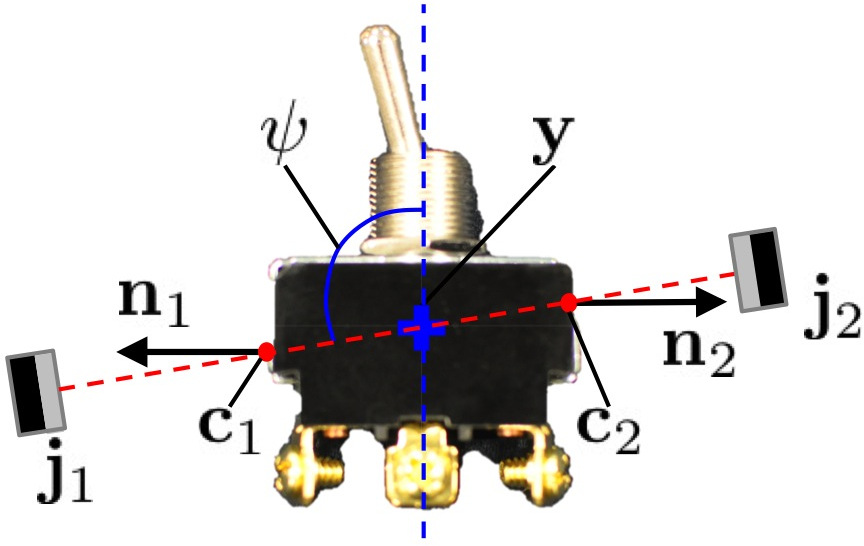
\includegraphics[width = 8.5cm, height = 5.25cm]{figures/bandit_grasp_model.jpg}
\caption{Illustration of our grasping model for parallel jaw grippers on a mechanical switch. Jaw placements are
illustrated by rectangles closing along the dashed line. A grasp plan centered at $\by$ (plus symbol) at angle $\psi$ consists of 2D locations for each of the parallel jaws $\bj_1$ and $\bj_2$. When following the grasp plan, the jaws contact the object at locations $\bc_1$ and $\bc_2$, and the object has outward pointing unit surface normals $\bn_1$ and $\bn_2$ at these locations. Together with the center of mass of the object $\bz$, these values can be used to determine the forces and torques that a grasp can apply to an object.}
\vspace*{-2ex}
\label{fig:grasp_model}
\end{figure}

\subsection{Candidate Grasp Model}
The grasp model is illustrated in Fig.~\ref{fig:grasp_model}. We formulate the MAB problem for planar objects using parallel-jaw grippers as modeled in Fig.~\ref{fig:grasp_model}. Similar to~\cite{mahler2015gp}, we parameterize a grasp using a {\it grasp axis}, the axis of approach for two jaws,  with jaws of width $w_j \in \mathbb{R}$ and a maximum width $w_g \in \mathbb{R}$. The two location of the jaws can be specified as $\mathbf{j}_1,\mathbf{j}_2 \in \mathbb{R}^2$, where $||\mathbf{j}_1 - \mathbf{j}_2||_2 \leq w_g$. We define a grasp consisting of the tuple $\Gamma = \lbrace \mathbf{j}_1, \mathbf{j}_2 \rbrace$. 

%We chose of the line of action model because perturbations to a surface resulting from shape uncertainty lead to changesa in the location of contact with a surface, and the line of action allows us to compute these new locations.

Given a grasp and an object, we define the {\it contact points} as the spatial locations at which the jaws come into contact with the object when following along the grasp axis, $\bc_1, \bc_2 \in \mathbb{R}^2$.
We also refer to the unit outward pointing surface normals at the contact points as $\bn_1, \bn_2 \in \mathbb{R}^2$, the object center of mass as $\bz \in \mathbb{R}^2$ and the friction coefficient as $\mu \in \mathbb{R}$.
%Together these form the set of grasp parameters that allows us to evaluate the forces and torques that a given grasp can apply to an object \cite{ferrari1992}. 

%\begin{figure}[ht!]
%\centering
%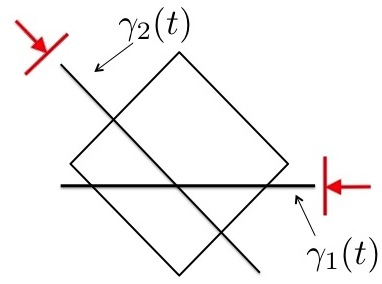
\includegraphics[width = 6cm, height = 4cm]{figures/Slide01.jpg}
%\caption{Illustration of a grasp plan $\Gamma$ composed of two lines of action, $\gamma_1(t)$ and $\gamma_2(t)$}
%\vspace*{-10pt}
%\label{fig:line_of_action}
%\end{figure}



\subsection{Sources of Uncertainty}
We consider uncertainty in object shape, object pose, grasp approach angle, and friction coefficient.
Fig.~\ref{fig:graphical_model} illustrates a graphical model of the relationship between these sources of uncertainty.
In this section, we describe our model of each source of uncertainty.

\begin{figure}[t!]
\centering
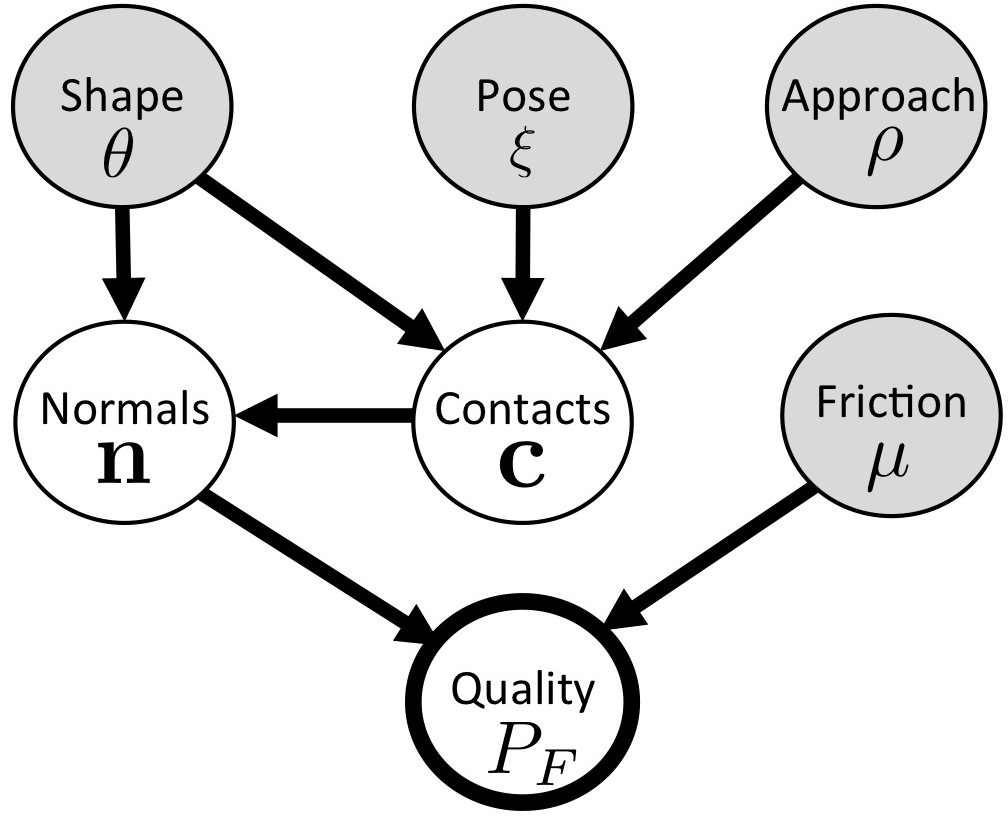
\includegraphics[scale=0.18]{figures/Graphical_Model.jpg}
\caption{A graphical model of the relationship between the uncertain parameters we consider. Uncertainty in object shape $\theta$, object pose $\xi$, and grasp approach angle $\rho$ affect the points of contact $\bc$ with the object and the surface normals $\bn$ at the contacts. Uncertainty in friction $\mu$ coefficient affects the forces and torques used to compute our quality measure, the probability of force closure $P_F$. The shaded nodes denote the observed values.  }
\vspace*{-10pt}
\label{fig:graphical_model}
\end{figure}

\subsubsection{Shape Uncertainty}

Uncertainty in object shape results from sensor imprecision and missing sensor data, which can occur due to transparency, specularity, and occlusions~\cite{mahler2015gp}.
Following ~\cite{mahler2015gp}, we represent the distribution over possible surfaces given sensing noise using a Gaussian process implicit surface (GPIS).
A GPIS represents a distribution over signed distance functions (SDFs).
A SDF is a real-valued function over spatial locations $f: \mathbb{R}^2 \rightarrow \mathbb{R}$ that is greater than 0 outside the object, 0 on the surface and less than 0 inside the object.
A GPIS is a Gaussian distribution over SDF values at a fixed set of query points $\mX = \{\bx_1, ... \bx_n\}, \bx_i \in \mathbb{R}^2$, $f(\bx_i) \sim \mN(\mu_{f}(\bx_i),\Sigma_{f}(\bx_i))$, where $\mu_{f}(\cdot)$ and $\Sigma_{f}(\cdot)$ are the mean and covariance functions of the GPIS~\cite{rasmussen2006}.
See Mahler et al. for details on how to estimate a mean and covariance function and sample shapes from a GPIS~\cite{mahler2015gp}.
For convenience, in later sections we will refer to the GPIS parameters as $\theta = \lbrace \mu_{f}(\bx), \Sigma_{f}(\bx) \rbrace$. 


\subsubsection{Pose Uncertainty}
In 2-dimensional space, the pose of an object $T$ is defined by a rotation angle $\phi$ and the two translation coordinates $\bt = (t_x, t_y)$, summarized in parameter vector $\mathbf{\xi} = (\phi, \bt)^T \in \mathbb{R}^3$.  We assume Gaussian uncertainty on the pose parameters $\mathbf{\xi} \sim \mN \left( \hat{\mathbf{\xi}}, \Sigma_{\xi} \right)$, where $\hat{\mathbf{\xi}}$ corresponds to the expected pose of the object. 

 
 \subsubsection{Approach Uncertainty}
In practice, a robot may not be able to execute a desired grasp $\Gamma = \lbrace \bj_i,\bj_2\rbrace$ exactly due to errors in actuation or feedback measurements used for trajectory following~\cite{kehoe2012estimating}.
We model approach uncertainty as Gaussian uncertainty around the angle of approach and centroid of a straight line grasp $\Gamma$.
Formally, let $\hat{\by} = \frac{1}{2} (\bj_1 + \bj_2)$ denote the center of a planned grasp axis and $\hat{\psi}$ denote the clockwise angle that the planned axis $\bj_1 - \bj_2$ makes with the y-axis of the 2D coordinate system on our shape representation.
We model uncertainty in the approach center as $\by \sim \mN(\hat{\by}, \Sigma_y)$ and uncertainty in the approach angle as $\psi \sim \mN(\hat{\psi}, \sigma_{\psi}^2)$.
To shorten notation, the remainder of this paper we will refer to the uncertain approach parameters as $\rho = \{\by, \psi \}$.
In practice $\Sigma_{y}^2$ and $\sigma_{\psi}^2$ can be set from repeatability measurements for a robot~\cite{mooring1986determination}.

 \subsubsection{Friction Uncertainty}
As shown in~\cite{hang2013a,zheng2005}, uncertainty in friction coefficient can cause grasp quality to significantly vary.
However, friction coefficients may be uncertain due to factors such as the presence of material between a gripper and an
object (e.g. dust, water, moisture), variations in the gripper material due to manufacturing tolerances, or due to a misclassification of the object surface to be grasped. We model uncertainty in friction coefficient as Gaussian noise, $\mu \sim \mN(\hat{\mu},\sigma_{\mu}^2)$.

 
\subsection{Grasp Quality}\label{sec:grasp_sample}
We measure the quality of a grasp using the notion of probability of force closure~\cite{kehoe2012estimating, kehoe2012toward, kim2012physically,weisz2012pose} given a grasp $\Gamma$. Force closure is considered as a binary-valued quantity $F$ that is 1 if the grasp can resist wrenches in arbitrary directions and 0 otherwise.
Let $\mW \in \mathbb{R}^3$ denote the contact wrenches derived from contact locations $\bc_1,\bc_2$, normals $\bn_1,\bn_2$, friction coefficient $\mu$, and center of mass $\bz$ for a given grasp and shape.
If the origin lies within the convex hull of $\mW$, then the grasp is in force closure~\cite{li1988task}.
We rank grasps using the probability of force closure given uncertainty in shape, pose, robot approach, and friction coefficient~\cite{christopoulos2007handling, kehoe2012toward}:

\vspace{-2ex}
\begin{align*}
	P_F(\Gamma_k) &= P \left(F = 1 | \Gamma_k, \theta, \xi, \rho, \mu \right).
\end{align*}
 
To estimate $P_F(\Gamma_k)$, we first generate samples from the distributions on $\theta, \xi, \rho,$ and $\mu$.
Using the relationships defined by the graphical model in Fig. \ref{fig:graphical_model}, we next compute the contact locations $\bc_1, \bc_2$ given a sampled SDF, pose, and grasp approach by ray tracing along the grasp axis defined by $\Gamma_k = \lbrace \bj_1,\bj_2 \rbrace$~\cite{mahler2015gp}.
We then compute the surface normals $\bn_1, \bn_2$ at the contacts using the gradient of the sampled SDF at the contact locations.
Finally, we use these quantities to compute the forces and torques that can be applied to form the contact wrench set $\mW$ and evaluate the force closure condition~\cite{li1988task}.

%After sampling a shape, pose, approach direction, and friction coefficient, we compute the contact locations $\bc_i$ and the surface normals $\bn_i$ using Bayes rule:
%
% \vspace{-2ex}
% \begin{align*}
% &p(\textbf{n}_i,\textbf{c}_i |\Gamma_k,\theta,\xi,\rho)=\\
% &p(\textbf{n}_i|\textbf{c}_i,\theta)p(\textbf{c}_i|\Gamma_k,\theta,\rho,\xi)
% \end{align*}
%
% 
%Mahler et al.describe how to draw shape samples from a GPIS model ~\cite{mahler2015gp}.
%We next sample from $p(\xi)$ and $p(\rho)$ to compute $p(\textbf{c}_i|\Gamma_k,\theta,\rho,\xi)$ via ray tracing along the grasp axis defined by $\Gamma_k = \lbrace \bj_1,\bj_2 \rbrace$~\cite{newcombe2011kinectfusion}.
%Then $p(\textbf{n}_i|\textbf{c}_i,\theta)$ corresponds to the normal vector at the sampled contact point.We use these quantities to compute the forces and torques that can be applied to form the contact wrench set $\mW$ and evaluate the force closure condition \cite{li1988task}.



\subsection{Objective}
\seclabel{objective}

Given the sources of uncertainty and their relationships as described above, the grasp planning objective is to find a grasp that maximizes the probability of force closure from a set of candidate grasps $\mG = \{\Gamma_1, ..., \Gamma_K\}$:

\vspace{-2ex}
\begin{align}
\Gamma^* &= \underset{\Gamma_k \in \mG}{\text{argmax }} P_F\left( \Gamma_k\right) \label{eq:old_problem_def}
\end{align}

% Since we only can approximate the probability of force closure, with samples drawn from the distribution $P_F(\Gamma)$ our objective is rewritten as: 

% \vspace{-2ex}
% \begin{align}
% \Gamma^* &\approx \underset{\Gamma \in \mG}{\text{argmax }} P\left( F = 1 | \Gamma, \theta, \xi, \rho, \mu \right) \label{eq:problem_def}
% \end{align}

One method to approximately find such a grasp is to exhaustively evaluate $P_F(\Gamma_k)$ for all grasp in $\mG$ using Monte-Carlo integration and then sort the plans by this quality metric.
We refer to this as a brute force approach. 
This method has been evaluated for shape uncertainty~\cite{christopoulos2007handling, kehoe2012estimating} and pose uncertainty~\cite{weisz2012pose} but may require many samples for each of a large set of candidates to converge to the true value.
More recent work has considered adaptive sampling to discard grasps that are not likely to be optimal without fully evaluating their quality~\cite{kehoe2012toward}.

To try and reduce the number of samples needed, we instead maximize the sum of $P_F$ values for each sampled grasp  $\Gamma_{k,t}$ at time $t$ up to a given time $T_s$:
\begin{align}
    \underset{\Gamma_{k,*} \in \mG}{\text{max }} \sum \limits_{t=1}^
    {T_s} P_F \left( \Gamma_{k,t}\right)  \label{eq:problem_def}
\end{align}
\noindent The goal is to perform as well as Equation~\ref{eq:old_problem_def} in as few samples as possible~\cite{srinivas2009gaussian}. We then formulate the  problem as a MAB model and compare two different Bayesian MAB algorithms, Thompson sampling and Gittins indices.

\section{Grasp Planning as a Multi-Armed Bandit}
We frame the grasp selection problem of \secref{objective} as a MAB problem.
Each arm corresponds to a different grasp, $\Gamma_k$, and pulling an arm corresponds to sampling from the graphical model in Fig. \ref{fig:graphical_model} and evaluating the force closure condition. Since force closure is a binary value, each grasp $\Gamma_k$ has a Bernoulli reward distribution with probability of force closure, $P_F(\Gamma_k)$.
In a MAB, we want to minimize cumulative regret which is an equivalent objective to the objective of Equation~\ref{eq:problem_def}.

The proposed algorithm is an anytime algorithm because it can be stopped at any point during its computation to return the current estimate of the best grasp or wait until a $95\%$ confidence interval is smaller than some threshold $\epsilon$. Using the quantile function of the beta distribution, $B$, we can measure the $95\%$ confidence interval as: 

\vspace{-2ex}
{\small
\begin{align}\label{eq:confidence}
B(0.025,\alpha_{k,t},\beta_{k,t}) \leq P_F(\Gamma_{k,t})) \leq B(0.975,\alpha_{k,t},\beta_{k,t}).
\end{align}
}
To summarize, the algorithm terminates and returns $\bar{k}$, or a grasp that has the highest estimated $P_F$ when 
$t \geq T_s $ or $|B(0.025,\alpha_{\bar{k},t},\beta_{\bar{k},t}) -
B(0.975,\alpha_{\bar{k},t},\beta_{\bar{k},t})| \leq \epsilon$.

\section{Simulation Experiments}
We used the Brown Vision Lab 2D dataset \cite{brown} of 2D objects as in \cite{christopoulos2007handling}.
We downsampled the silhouette by a factor of 2 to create a 40 x 40 occupancy map, which contained 1 if the object was
observed and 0 if it was not observed. We computed a quadtree representation of the SDF and removed information about
the SDF on grid cells corresponding to uniformly chosen quadtree cells to simulate localized uncertainty in shape perception.
We then construct a GPIS using the same method as proposed in~\cite{mahler2015gp}.
The noise parameters in approach, pose, and friction coefficient were set to the following variances: $\sigma_{\psi}^2 = 0.2$ rads$^2$, $\sigma_{\by}^2 = 3$ grid cells$^2$, $\sigma_{\mu}^2 = 0.4$, $\sigma_{\phi}^2 = 0.3$ rads$^2$ and $\sigma_{\bt}^2 = 3$ grid cells$^2$.
We  performed experiments for the case of two hard contacts in 2-D.
We drew random grasps $\Gamma$ by uniformly sampling the angle of the grasp axis around a circle with radius $\sqrt{2}
M$, where $M$ is the dimension of the workspace, and then sampling the circle's origin from a zero mean Gaussian with
variance 10 units$^2$. All experiments were run on a machine with OS X with a 2.7 GHz Intel core i7 processor and 16 GB
1600 MHz memory in Matlab 2013b. 
Figure \ref{fig:shape_samples} displays examples of GPIS models using the GPIS-Blur method~\cite{mahler2015gp}
as well as resulting grasp samples.

\subsection{Multi-Armed Bandit Experiments}
For our experiments, we consider selecting an optimal grasp among $|G| = 1000$ candidates per object. We draw samples from our
graphical model using the technique described in Sec.  \ref{sec:grasp_sample}. We calculated the expected performance
over 100 randomly selected shapes in the Brown Vision Lab 2D dataset and for the grasps planned by Thompson sampling,
Gittins indices, iterative pruning~\cite{kehoe2012toward} and uniform allocation. Uniform allocation selects a grasp at
random from the set to sample the next candidate and thus does not use any prior information. Iterative pruning prunes
grasps every 1000 iterations based on lowest sample mean and removes 10$\%$ of the current grasp set.  We set the
discount factor $\gamma =0.98$ for the Gittins method, which was the highest we could compute in a reasonable amount of
time due to the exponential growth in computation time with respect to $\gamma$~\cite{gittins2011multi}. 

In Fig. \ref{fig:grasp_quality}, we plot time $t$ vs. $P(\Gamma_{\bar{k},t})$/$P(\Gamma^*)$, the normalized probability
of force closure for the grasp returned by the algorithm.  Non-MAB methods such as uniform sampling and iterative
pruning (eliminating candidates grasp based on sample mean) eventually converge to within 3$\%$ of the optimal grasp,
requiring approximately 40,000 and 20,000 iterations.  Gittins indices and Thompson sampling  perform significantly
better, converging after only 4000 iterations. In Fig. \ref{fig:shape_samples}, we select a stopping time $T_s=10,000$,
which corresponds to 10 samples per grasp on average, and for each method visualize the grasp returned,
$\Gamma_{\bar{k},10,000}$.

The time per iteration is $t_{i} = t_{a}+t_{p}$, where $t_{a}$ is the time to decide which arm to pull next and $t_{p}$ is the time taken to draw a sample from the graphical model in Fig. \ref{fig:graphical_model}. The time per iteration for Thompson sampling, Gittins indices, iterative pruning and uniform allocation is $31.6$, $31.2$, $30.4$ and $30.2$ ms. Most of $t_{i}$ is dominated by sampling time, since $t_{p} \approx 30$ ms. Sampling from our graphical model in Fig. \ref{fig:graphical_model} involves drawing samples form a GPIS, a high dimensional Gaussian, and evaluating the probability of force closure metric. 
The MAB algorithm can also be terminated when the $95\%$ confidence interval around the returned grasp (see Equation
\ref{eq:confidence}) is below a set threshold $\epsilon$ in size. We plot the algorithm's confidence intervals around the returned grasp $P_F(\Gamma_{\bar{k}})$ vs. the number of samples drawn in Fig. \ref{fig:confidence} for the Gittins indices, Thompson sampling, iterative pruning~\cite{kehoe2012toward} and uniform allocation.  As illustrated, the confidence interval for Thompson sampling and Gittins indices converges at a faster rate than the other two methods. 


\begin{figure}[t!]
\centering
\includegraphics[scale=1]{matlab_figures/confidence_bounds.jpg}
\caption{ Number of samples versus the algorithm's $95\%$ confidence intervals from Eq. \ref{eq:confidence} on the probability of force closure of the best estimated grasp after $t$ samples using uniform allocation, iterative pruning, Gittins indices, and Thompson Sampling. The values are averaged over 100 independent runs on randomly selected objects from the Brown Vision 2D Dataset~\cite{brown} with 1,000 candidate grasps for each object. An increasingly narrow confidence interval indicates that the algorithm allocated an increasing number of samples to its estimate of the best grasp. }

\vspace*{-15pt}
\label{fig:confidence}
\end{figure}


\begin{figure*}%
\label{fig:shape_examples}
    \centering
    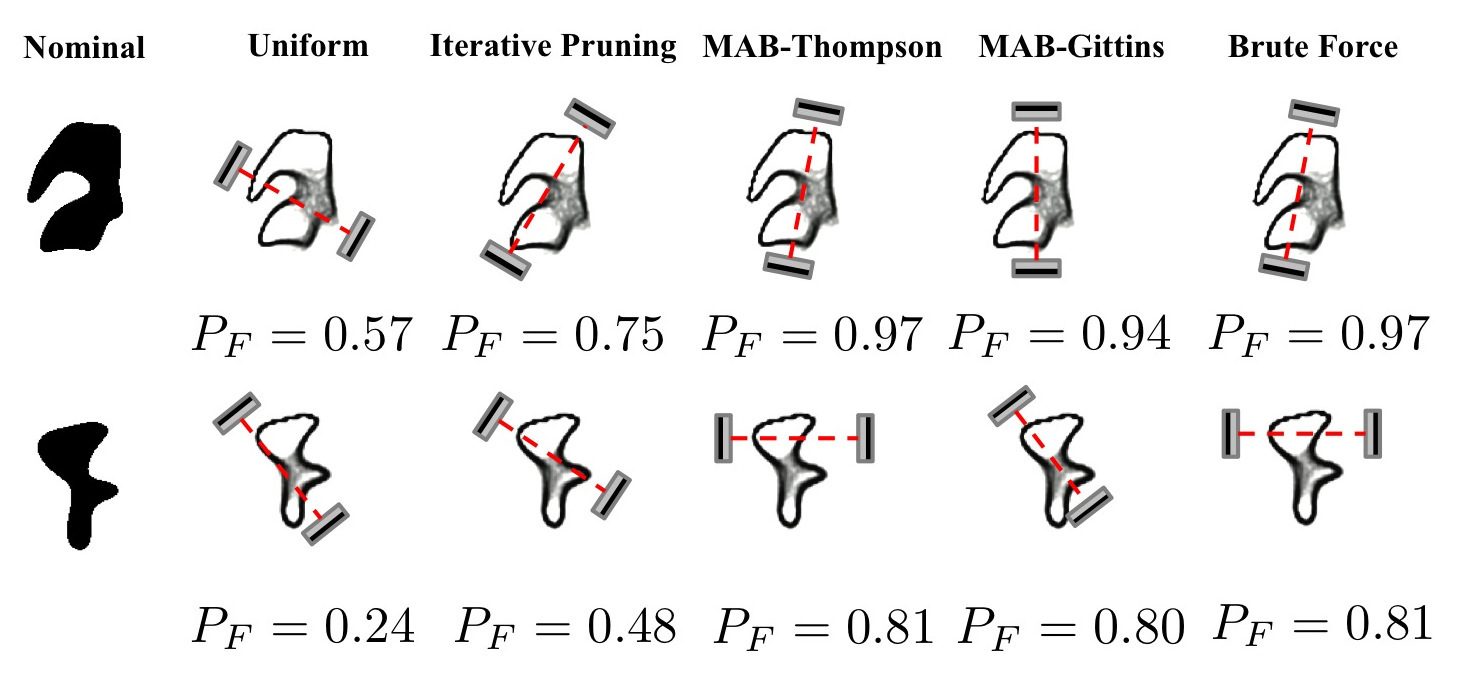
\includegraphics[width=16.5cm]{figures/shapes.jpg}%
    \caption{Grasps with the highest estimated probabilty of force closure $P_F$ after 10,000 samples using uniform
    allocation, iterative pruning, Gittins indices, and Thompson sampling on two objects from the Brown 2D dataset
\cite{brown}. For reference, we also show the grasp with highest $P_F$ after brute force evaluation using 100,000
samples and the nominal shape. The candidate grasp set was of size $|\mG|=1000$ for each object. We visualize the GPIS
representation of the imposed object shape uncertainty using GPIS-Blur~\cite{mahler2015gp}, which causes more uncertain areas to appear more blurry.}%
    \label{fig:shape_samples}%
\end{figure*}

\begin{figure}[ht!]
\centering
\includegraphics[scale=1]{matlab_figures/worst_case-02.jpg}
\caption{ \footnotesize 
	Number of samples versus the probability of force closure of the best estimated grasp after $t$ samples $P_F(\Gamma_{\bar{k}, t})$ using uniform allocation, iterative pruning, Gittins indices, and Thompson sampling over 1,000 candidate grasps when samples are ordered such that many perturbations that do result in force closure are given to the algorithm initially for grasps of low quality.
	The normalized $P_F$ is the ratio of the best estimated grasp at iteration $t$, $P_F(\Gamma_{\bar{k}, t})$, to the highest $P_F$ in the candidate grasp set $P_F(\Gamma^*)$ averaged over 100 independent runs on randomly selected objects from the Brown Vision 2D Dataset~\cite{brown}.
 	The highest quality grasp was determined by brute force search over all candidate grasps (which required 10x  more time than any of these methods~\cite{kehoe2012toward}).
 	The results suggest that when samples are misleadingly ordered, the best policy is uniform allocation.}
\vspace*{-10pt}
\label{fig:worst_case}
\end{figure}
\subsection{Sensitivity Analysis }\label{sec:sensitivity}
We also analyze the performance of Thompson sampling under variations in noise from friction coefficient uncertainty, shape uncertainty, rotational pose, and translation pose.
We increase the variance parameters across a set range for each parameter to simulate low, medium and high levels of noise.
All experiments were averaged across 100 objects randomly selected  from the Brown dataset with $|\mG| = 1000$.

For the friction coefficient, we varied $\sigma^2_{\mu}$ across the values $\lbrace 0.05, 0.2, 0.4 \rbrace$.
As illustrated in Table 1, the performance of the bandit algorithm remains largely unchanged, with typical convergence
to zero in simple regret in less than 5000 iterations.

For rotational uncertainty in pose, we varied $\sigma^2_{\phi}$ across the set $\lbrace 0.03, 0.12,0.24\rbrace$ radians$^2$. As illustrated in Table 1, the performance of the bandit algorithms is affected by the change in rotation. Increase in variance to $0.24$ radians$^2$  causes the  simple regret to not converge until around 6432 samples or an average of 6.4 samples per grasp. 

For translational uncertainty in pose, we varied $\sigma^2_{\bt}$ in the range of $\lbrace 3,12, 24 \rbrace$ units$^2$ (on a 40 x 40 unit workspace). Our results indicate that the performance of the bandit algorithms is affected by the change in rotation and an increased noise of $\sigma^2_{\bt} = 24$ causes the algorithm to not converge until 8763 evaluations for Thompson sampling. 



\subsection{Worst Case}
The MAB algorithms use the observations of samples drawn to decide which grasp to sample next from. To show worst case performance under such a model, we sorted the quality of all 1000 grasps offline and arranged the order of samples, so that the top 500 grasps have samples drawn in the order of worst to best and the bottom 500 grasps have samples drawn in order of best to worst. This provides misleading observations to the bandit algorithms. We demonstrate in Fig. \ref{fig:worst_case} a case where the observations are misleading. As illustrated in Fig. \ref{fig:worst_case}, all methods are affected by worst case performance. The results suggest that, when the observations are misleading, the preferred policy is uniform allocation of grasp samples.






\begin{table}[t]
\centering
\begin{tabular}{ R{1.75cm}||R{1.65cm}|R{1.65cm}|R{1.65cm}  }
 %\hline
 %\multicolumn{4}{|c|}{Sensitivity Analysis for Convergence to Best Grasp for Thompson sampling} \\
 %\hline 
 & \multicolumn{3}{c}{$\#$ of Samples Until Convergence} \\
 \hline
\specialcell{\bf Uncertainty\\ \bf Type} & \specialcell{\bf Low\\ \bf Uncertainty} & \specialcell{\bf Medium \\ \bf Uncertainty} & \specialcell{\bf High\\\bf Uncertainty}\\
 \hline
Orientation $\sigma_{\phi}$ & 4230 & 5431 &  6432\\
Position $\sigma_{\bt}$ & 4210    & 5207 &  8763\\
Friction $\sigma_{\mu}$ &  4985  & 4456   & 4876\\
 %\hline
\end{tabular}
   \caption { \footnotesize  Number of iterations until convergence to within $3\%$ of grasp with the highest estimated probability of force closure $P_F$ for Thompson sampling under uncertainty in the object orientation $\sigma_{\phi}^2 = \lbrace 0.03,0.12, 0.24 \rbrace$ radians$^2$,  uncertainty in the object position $\sigma_{\bt}^2 = \lbrace 3, 12, 24 \rbrace$ units$^2$, and uncertainty in friction coefficient $\sigma_{\mu}^2 = \lbrace 0.05,0.2, 0.4 \rbrace$ on a 40$\times$40 grid averaged over 100 independent runs on random objects from the Brown Vision 2D Dataset. High variances in position and orientation uncertainty increases the amount of iterations needed for the bandit algorithm to converge.
   }
		\tablabel{opt-p-comparison}
\vspace*{-20pt}
\end{table}


\section{Discussion and Future Work } 

In this work, we proposed a multi-armed bandit approach to efficiently identify high-quality grasps under uncertainty in shape, pose, friction coefficient and approach. 
A key insight from our work is that exhaustively sampling each grasp is inefficient, and we found that a MAB approach gives priority to promising grasps and can reduce computational time. Initial results have shown MAB algorithms to outperform the methods of prior work, uniform allocation and iterative pruning  ~\cite{kehoe2012estimating,kehoe2012toward} in terms of finding a higher quality grasp faster.
However, as shown in Fig. \ref{fig:worst_case} there are some pathological cases that can mislead bandit algorithms to focus samples on the wrong grasps.
Fortunately, the probability of many successive samples being misleading rapidly approaches zero as the time horizon is increased.

In future work, we plan to scale our method to 3D objects. This could substantially increase the number of candidate grasps, further motivating the use of cloud computing. Glazebrook and Wilkinson showed that the Gittins index method could be parallelized by simply dividing the arms into $M$ subsets, where $M$ is the number of cores, and solving each MAB separately. \cite{glazebrook2000index}. A similar method could also be done for Thompson sampling. Another promising scheme for parrallelizing the MAB, is to have the algorithm not sample one arm at each iteration but $M$. We will explore both of these approaches in future work.

\section{Acknowledgments} 
This work is supported in part by the U.S. National Science Foundation under Award IIS-1227536, NSF-Graduate Research Fellowship, and by grants from Google. 
We thank the AMPLab, UC Berkeley and our colleagues who gave feedback and suggestions, in particular Sanjay Krishnan, Peter Bartlett, Steve McKinley and Dylan Hadfield-Menell.

\bibliographystyle{IEEEtranS}
\bibliography{references}



\end{document}
